\label{procedimentos}

O presente trabalho pode ser classificado quanto a diversos aspectos. Em termos de objetivos, a pesquisa se classifica como \textit{pesquisa exploratória}, pois conceitos e modelos existentes são utilizados e experimentados a fim de se elaborar uma aplicação na qual poderemos desfrutar dos modelos para um subconjunto de imagens. Nenhum novo modelo foi proposto. Quanto aos procedimentos técnicos, esta pesquisa se classifica como \textit{pesquisa experimental}. Apesar de a coleta e análise de resultados estatísticos minuciosos e rebuscados não serem o foco principal do trabalho, algumas métricas são adotadas, medidas e analisadas. Portanto, com a característica principal do trabalho sendo a de experimentar sobre o trabalho anterior de terceiros, a pesquisa experimental se encaixa mais confortavelmente com o escopo do trabalho.

\section{Fluxo de desenvolvimento}

Nesta parte do trabalho é definido o fluxo no qual a proposta foi implementada, desde o princípio majoritariamente teórico, até a parte mais prática, onde é testado de fato, modelos de redes geradoras adversárias. O diagrama da figura \ref{fig:fig9} ilustra as fases e as subseções em sequência, detalham um pouco mais a fundo a intenção e objetivos de cada uma das fases.

\begin{figure}[H]
    \centering
    \caption{Diagrama de fluxo dos procedimentos metodológicos planejados para a realização e avaliação do trabalho e de seus resultados.}
    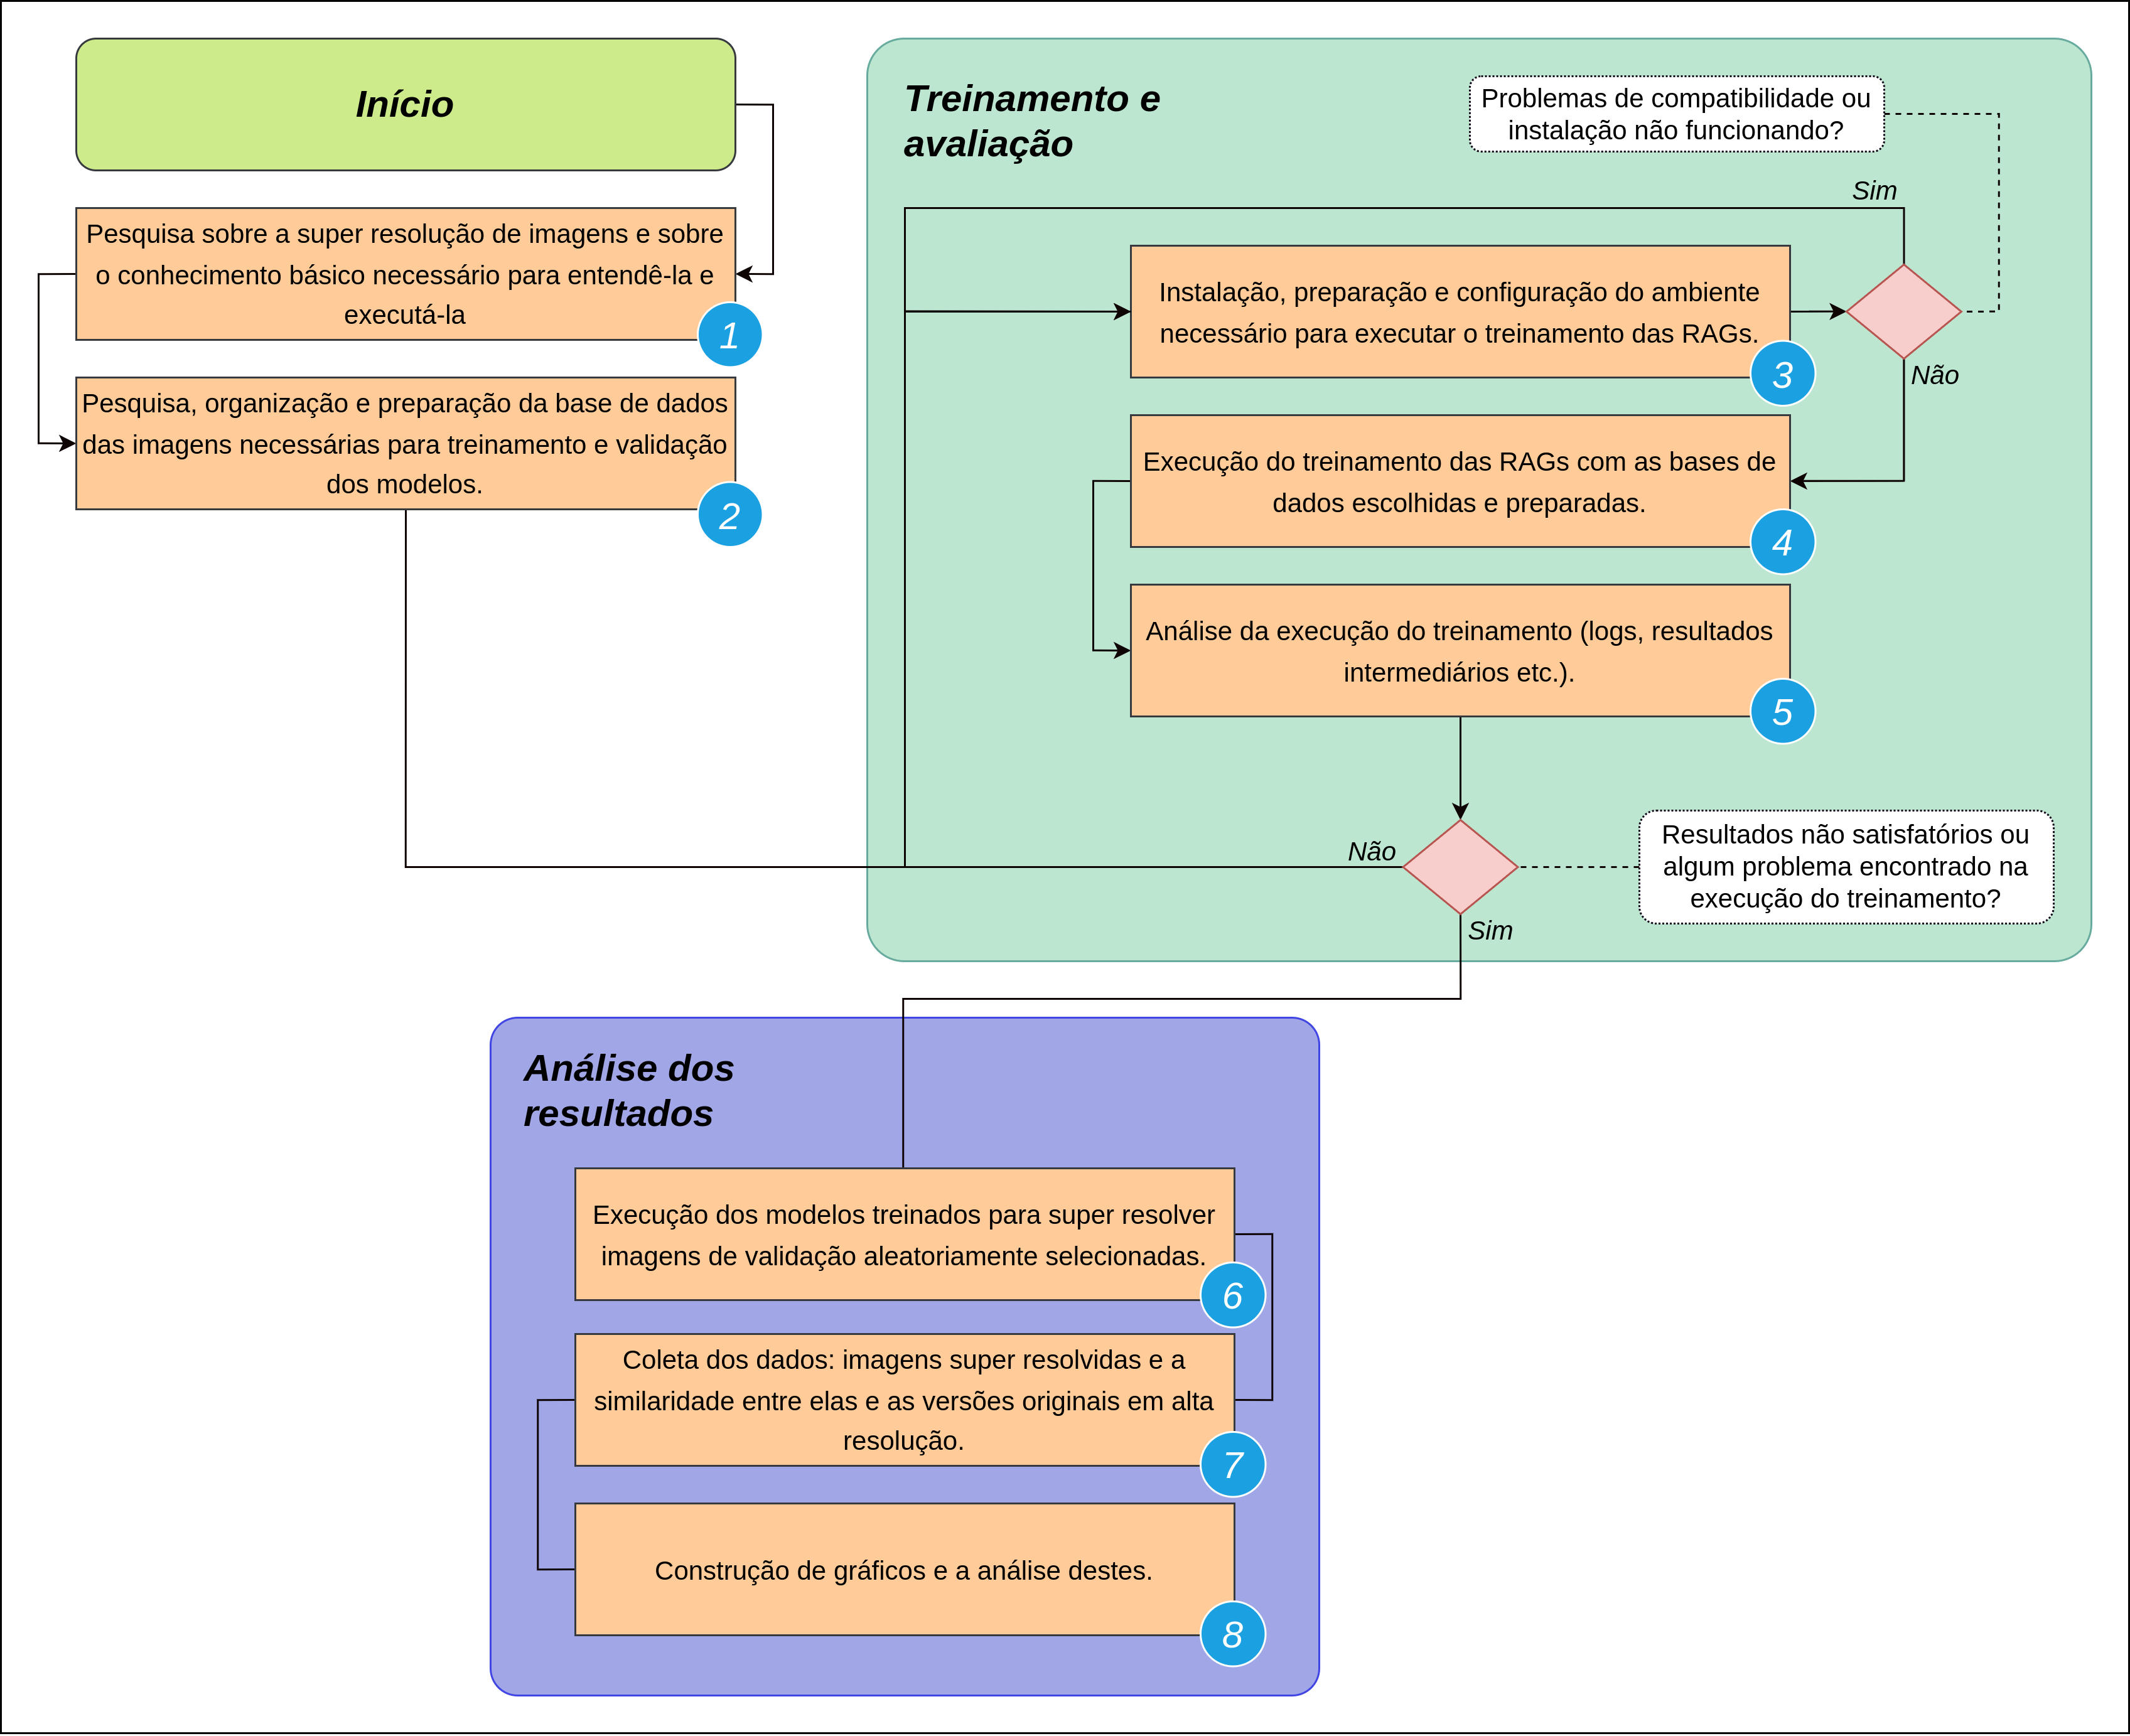
\includegraphics[width=14cm]{fig/flow_diagram_development.png}
    \legend{Fonte: autor.}
    \label{fig:fig9}
\end{figure}

\subsection{Pesquisa sobre super resolução de imagens (etapa n\textsuperscript{o} 1)}
\label{sec:procedimentos:pesquisa-super-resolucao}

Esta fase representa toda a pesquisa não necessariamente planejada que ocorreu anteriormente e durante as fases práticas de experimentação. Ela envolveu desde questões teóricas sobre as tecnologias desenvolvidas como resoluções de dúvidas e problemas que foram encontrados no caminho de pesquisa e desenvolvimento. Durante as fases finais, uma quantidade grande de dúvidas, naturalmente surgiu. Esta etapa da metodologia engloba também as pesquisas para sanar tais dúvidas de implementação, implantação, testes e validação, não se restringindo apenas à pesquisa preliminar do trabalho.

\subsection{Pesquisa, organização e preparação das imagens (etapa n\textsuperscript{o} 2)}
\label{sec:procedimentos:organizacao-preparacao-imagens}

Dados são requisitos básicos para se treinar modelos de redes neurais. No caso deste trabalho, especificamente  imagens científicas de áreas médica e astronômica são utilizadas. Existem bases de dados famosas e acessíveis para ambas as aplicações como as disponíveis nos sites \textit{OpenfMRI} e no \textit{Catálogo de dados do governo dos Estados Unidos}. O trabalho desta etapa consistiu na classificação e segregação das imagens obtidas nestas fontes e preparação para treinar e alimentar os modelos. 

Esta preparação consistiu em algumas etapas:

\begin{enumerate}
    \item Dimensionar as imagens de acordo com a necessidade e recursos disponíveis. Imagens maiores requerem mais poder computacional para serem processadas e mais tempo de treinamento dos modelos. No caso deste trabalho, ambos são limitados, portanto a resolução das imagens precisa ser reduzida.
    
    \item Recortar as imagens para uma resolução consistente, i.e., todas imagens com mesma altura e mesma largura. Esta consistência é importante, pois a dimensão dos parâmetros da rede convolucional não se adapta ao tamanho da imagem de entrada.
    
    \item Gerar imagens de baixa resolução a partir das imagens obtidas nas fases 1 e 2. O conjunto das imagens dimensionadas e recortadas com as imagens de baixa resolução formou a base de dados para o treinamento da RAG. Estas imagens com resolução reduzida, devem ser alimentadas ao modelo para que este produza uma imagem de resolução alta. Estas imagens são, posteriormente comparadas com as imagens originais para tomar-se conhecimento da eficiência e precisão do método utilizado.
    
\end{enumerate}

No fim da preparação destes dados, que não são dedicados especificamente ao uso em redes adversárias geradoras, uma nova base de dados nasce, preparada para este estilo de modelo.

\subsection{Treinamento e avaliação (etapas n\textsuperscript{o} 3, 4 e 5)}
\label{sec:procedimentos:treinamento-avaliacao}

Repare que no diagrama (\ref{fig:fig9}) esta fase consiste em duas sub-etapas. Estas sub-etapas sãos repetidas caso o resultado não seja satisfatório. Eventualmente algum parâmetro de treinamento pode ser alterado a fim de obtermos um resultado idôneo.

\subsection{Instalação, preparação e configuração do ambiente (etapa n\textsuperscript{o} 3)}

Nesta etapa, todo software necessário para o treinamento e execução dos modelos são instalados e configurados, atentando-se aos diferentes níveis de compatibilidades entre as variadas partes envolvidas. Esta fase é suscetível a muitos problemas de equivalência entre versões de softwares e justamente por isso, erros são comuns nas execuções. Estas dificuldades são as razões por trás do laço superior nesta fase, retornando para ela mesma: caso a instalação dê errado, uma nova tentativa, com configurações diferentes é realizada.

\subsubsection{Execução do treinamento das RAGs (etapa n\textsuperscript{o} 4)}

Nesta etapa, executa-se e experimenta-se com as redes generativas adversárias escolhida. É colocado em prática o que foi definido até então, somente na teoria. Em alguns trechos desta etapa é necessário deixar o modelo treinando e esta etapa consume bastante tempo. Por este motivo, é preciso prestar bastante atenção nas limitações de recursos durante a etapa de preparação das imagens (seção \ref{sec:procedimentos:organizacao-preparacao-imagens}). 

Modelos existentes foram utilizados. Tais modelos estão disponíveis em repositórios de aprendizado de máquina e são treinados em bases de imagens genéricas, como fotos cotidianas, imagens de animais, paisagens etc. Estes modelos existentes foram treinados, neste trabalho, com a mesma técnica dos modelos especificamente treinados para o objetivo deste trabalho: verificar a qualidade com a qual ele produz imagens médicas e astronômicas de alta resolução, mesmo não sendo treinado especificamente para este contexto e escopo.

\subsubsection{Análise da execução do treinamento (etapa n\textsuperscript{o} 5)}

Aqui, são julgados, os treinamentos obtidos pelas experimentações, e de acordo com estes, a decisão de prosseguir ou regredir alguns passos para refazer experimentos é tomada. Com um treinamento satisfatório, pula-se para a próxima fase. Caso contrário, a fase anterior é executada novamente, calibrando os parâmetros de treinamento. Todo o processo de treinamento e seus dados colhidos são documentados, independentes se satisfazem ou não os objetivos. Esta fase pode também retornar à fase de número 3, caso os resultados não estejam de acordo com o esperado.

\subsection{Execução dos modelos treinados (etapa n\textsuperscript{o} 6)}
\label{sec:procedimentos:execucao-modelo-treinado}

Nesta etapa, os modelos que foram treinados com sucesso nas etapas anteriores, são executados com as imagens obtidas na etapa de organização (seção \ref{sec:procedimentos:organizacao-preparacao-imagens}).

\subsection{Coleta de dados (etapa n\textsuperscript{o} 7)}
\label{sec:procedimentos:coleta-dados}

Aqui, os dados são coletados: imagens que foram super resolvidas e também a similaridade entre estas e suas respectivas versões originais em alta resolução. Para tornar esta fase mais eficiente, scripts são utilizados para não só coletar os dados, como também analisá-los e organizá-los.

\subsection{Construção de gráficos e análise destes (etapa n\textsuperscript{o} 8)}
\label{sec:procedimentos:graficos-analise}

Com um volume grande de imagens, sem uma maneira visual de compreender os resultados, pouco pode-se dizer sobre os resultados. Então nesta fase, os dados coletados na etapa anterior (seção \ref{sec:procedimentos:coleta-dados}) são plotados, visualizados e comentados. 

\section{Materiais e métodos}
Esta seção descreve os materiais utilizados no desenvolvimento do trabalho. No caso presente, o material se restringe ao hardware utilizado para toda integração, treinamento e avaliação. Também nesta seção, são descritos quais métodos de avaliação das imagens são utilizados e também, através de qual ferramenta ou biblioteca estes são acessíveis. 

\subsection{Descrevendo o hardware disponível}
\index{Treinamento}

Para treinar o modelo, um computador esteve disponível. A especificação de seu hardware está contida na tabela abaixo:

\begin{table}[H]
    \centering
    \caption{Tabela de descrição do hardware}
    \begin{tabular}{|l|l|} \hline
        \textbf{Item}            & \textbf{Descrição}                    \\ \hline
        CPU                      & Intel i7 Octa Core                    \\ \hline
        Memória RAM              & 16GB                                  \\ \hline
        Memória de Vídeo         & 2GB                                   \\ \hline
        Modelo da placa de vídeo & GeForce MX350                         \\ \hline
        Disco                    & 512GB (apenas 90GB disponível)        \\ \hline
        Sistema operacional      & Windows 10 e Ubuntu 24.04 disponível  \\ \hline
    \end{tabular}
    \vspace{0.3cm}
    \legend{Fonte: Autor.}
    \label{tab:my_label}
\end{table}

A placa de vídeo apresentada (GeForce GT920M) é um modelo de computadores portáteis voltada para jogos. Uma informação importante de se documentar, é sua quantidade de Núcleos \textit{CUDA}\index{CUDA} conhecidos popularmente pelo termo em inglês \textit{Cuda Core}. Os núcleos \textit{CUDA} são os núcleos de processamento de instruções das \textit{GPUs} da \textit{NVIDIA}, conceito bem parecido com o conceito de núcleos de processadores \cite{ryles_what_2022}. A placa em questão possui compatibilidade com \textit{CUDA}, um requisito indispensável, e possui 384 núcleos \textit{CUDA} \cite{nvidia_geforce_2022, technical_city_nvidia_2022}. Esta placa de vídeo de entrada possui 96 vezes mais núcleos que a CPU disponível.

O hardware descrito, está distante de ser o ideal para o treinamento de um modelo complexo e exigente em termos de recursos, como é o caso do modelo descrito e utilizado neste trabalho. Treinamentos do tipo costumam ser feitos em servidores dedicados, com processadores poderosos e grandes quantidades de memória RAM e memória de vídeo (VRAM).

Por causa desta limitação de recursos, é preciso recorrer à alternativas a nível de software, como descrito na seção \ref{sec:prep-imgs}.

\subsection{Métodos de avaliação de similaridade entre imagens}
\label{aval-similarity-images}

Como dito na seção \ref{sec:qualidade-imagem}, existem formas quantitativas de avaliar a qualidade de imagens. Um pequeno programa foi desenvolvido para lidar com essa tarefa de forma automatizada \cite{vasconcelos_leonamtvimage-similarity-scripts_2023}. O programa executa em linha de comando, recebendo como parâmetros as duas imagens e os algoritmos de similaridade que será utilizado. O software tem os seguintes algoritmos de similaridade disponíveis: MSE, RMSE, PSNR, UQI, SSIM, ERGAS, SCC, RASE, SAM, MSSSIM e VIFP. Para o escopo deste trabalho, serão utilizados os algoritmos MSE, RMSE, PSNR e ERGAS.
